\apendice{Plan de Proyecto Software}

\section{Introducción}
La primera fase de un proyecto es la planificación del mismo, la fase más importante para poder estimar el trabajo, el tiempo y el dinero que va a suponer su realización. En este anexo podremos ver detalladamente cada una de las estimaciones realizadas para valorar más tarde el desarrollo y los costes que verdaderamente han sido producidos.
La planificación del proyecto a su vez, se desglosa en dos estudios:
\begin{itemize}
    \item {La planificación temporal}
    \item {El estudio de viabilidad económica y legal}
\end{itemize}



\section{Planificación temporal}
La planificación temporal se ha llevado a cabo a través de un repositorio específico en Github llamado XacoMeterII-Twitter con url: \url{https://github.com/nataliafraanco/XacoMeterII-Twitter}\\
Para relizar el control del proyecto se ha utilizado la herramienta Zenhub de Github. Con ésta, se ha dividido el proyecto en \textit{sprints}, con una duración cada uno de dos semanas, que a su vez se dividen en diferentes tareas a resolver.\\
La visualización de las tareas realizadas en cada sprint y su resolución se ha llevado a cabo a través de \textit{"Burndown reports"}, los cuales consisten en mostrar gráficamente la evolución del proyecto en cada uno de los \textit{sprints}.

\subsection{Sprint 0 : 28 Septiembre 2022 - 13 Octubre 2022}
El primer \textit{sprint} fue una toma de contacto con el trabajo. Entender qué es lo que quería hacer y qué necesitaba para ello, es decir, investigar sobre cada una de las herramientas necesarias y decidir cuáles iba a implementar, antes comparando todas las opciones.
Además se montó un inicio de lo que podría ser el origen de la página web, aunque al ser solo un boceto se modificaría en otros \textit{sprints} más adelante.
Además, en un primer momento me propuse empezar a trabajar con la API de Twitter, pero no contabilicé bien los tiempos e invertí todo mi tiempo en la búsqueda de la información necesaria para comenzar, por lo que los anteriores issues decidí realizarlos en el siguiente \textit{sprint}.
En el siguiente gráfico que se muestra a continuación, se puede ver mi evolución dentro del \textit{sprint}.
\imagen{Sprint0}{Sprint 0 - Gráfica informe de evolución}


\tablaSmallSinColores{Sprint 0 - Tabla de tareas y tiempos}{p{5cm} p{4cm} p{4cm}}{Sprint 0 - Tabla de tareas y tiempos}
{
  \multicolumn{1}{p{5cm}}{\textbf{Tareas realizadas}} & \textbf{Tiempo estimado (h)} & \textbf{{Tiempo empleado (h)}}\\
 }
 {
Investigación sobre herramientas  & \multicolumn{1}{r}{10}& \multicolumn{1}{r}{15}\\
Elección de herramientas  & \multicolumn{1}{r}{3}& \multicolumn{1}{r}{3}\\
Inciciación con LateX  & \multicolumn{1}{r}{3}& \multicolumn{1}{r}{2}\\
Esquema página web  & \multicolumn{1}{r}{8}& \multicolumn{1}{r}{5}\\
Implementar API Twitter  & \multicolumn{1}{r}{5}& \multicolumn{1}{r}{-}\\\hline
\textbf{Tiempos totales}  & \multicolumn{1}{r}{29} & \multicolumn{1}{r}{25}\\
}


\subsection{Sprint 1 : 13 Octubre 2022 - 26 Octubre 2022}
En este \textit{sprint} he completado las tareas que no completé en el \textit{sprint} 0.
Implementé una manera de utilizar la API de Twitter para poder abstraer los datos, y en un principio lo desarrollé mediante la herramienta \textit{Tweepy} y con unos permisos esenciales.
La tutora consiguió obtener los permisos necesarios para tener una cuenta educativa con sus datos, pero a la hora de introducir las credenciales causaba varios fallos, los cuales me llevaron bastante tiempo arreglar y no llegué a tiempo para terminarlos en este \textit{sprint}, por lo que se terminó en el siguiente.
\imagen{Sprint1}{Sprint 1 - Gráfica informe de evolución}

\tablaSmallSinColores{Sprint 1 - Tabla de tareas y tiempos}{p{5cm} p{4cm} p{4cm}}{Sprint 1 - Tabla de tareas y tiempos}
{
  \multicolumn{1}{p{5cm}}{\textbf{Tareas realizadas}} & \textbf{Tiempo estimado (h)} & \textbf{{Tiempo empleado (h)}}\\
 }
 {
Implementar API Twitter(Sprint 0)  & \multicolumn{1}{r}{5}& \multicolumn{1}{r}{30}\\
Acceder con credenciales educativas  & \multicolumn{1}{r}{21}& \multicolumn{1}{r}{20}\\
Selección de campos a obtener  & \multicolumn{1}{r}{2}& \multicolumn{1}{r}{-}\\\hline
\textbf{Tiempos totales}  & \multicolumn{1}{r}{28} & \multicolumn{1}{r}{50}\\
}


\subsection{Sprint 2 : 26 Octubre 2022 - 9 Noviembre 2022}
En el este tercer \textit{sprint}, se continuó intentando introducir las credenciales educativas. Tras varias reuniones con los tutores, encontramos el fallo y conseguimos continuar. Se aplicaron los cambios, se decidieron los parámetros que se iban a utilizar y cómo incluirlos para obtener los resultados esperados de la API de Twitter para un futuro uso en la aplicación.
En este \textit{sprint} se intentó avanzar lo que llevaba atrasado debido a la parada que me causó el fallo con las credenciales educativas y decidí crear la base de datos.\\
Además, se creó una nube de palabras con los datos obtenidos de la API para poder tener algo visual y ver que funcionaba todo correctamente, aunque aún no se había decidido si esa nube de palabras constaría en el proyecto final.\\
Se comenzó también a implementar varias funciones que insertasen los datos obtenidos en la base de datos. Al ser mucho trabajo para este \textit{sprint}, continué con estas tareas en los siguientes \textit{sprints}.
\imagen{Sprint2}{Sprint 2 - Gráfica informe de evolución}
\tablaSmallSinColores{Sprint 2 - Tabla de tareas y tiempos}{p{5cm} p{4cm} p{4cm}}{Sprint 2 - Tabla de tareas y tiempos}
{
  \multicolumn{1}{p{5cm}}{\textbf{Tareas realizadas}} & \textbf{Tiempo estimado (h)} & \textbf{{Tiempo empleado (h)}}\\
 }
 {
Acceder con credenciales educativas (Sprint 1)  & \multicolumn{1}{r}{40}& \multicolumn{1}{r}{15}\\
Selección de campos a obtener (Sprint 1)  & \multicolumn{1}{r}{2}& \multicolumn{1}{r}{2}\\
Elección de base de datos y creación  & \multicolumn{1}{r}{13}& \multicolumn{1}{r}{25}\\
Gráfico con nube de palabras  & \multicolumn{1}{r}{3}& \multicolumn{1}{r}{5}\\
Verificación de filtros API Twitter  & \multicolumn{1}{r}{3}& \multicolumn{1}{r}{4}\\
Insertar datos en la base de datos  & \multicolumn{1}{r}{8}& \multicolumn{1}{r}{15}\\\hline
\textbf{Tiempos totales}  & \multicolumn{1}{r}{69} & \multicolumn{1}{r}{66}\\
}

\subsection{Sprint 3 : 9 Noviembre 2022 - 23 Noviembre 2022}
Este \textit{sprint} se dedicó totalmente a la inserción de datos en la base de datos. 
Se consiguió que la aplicación, una vez ejecutada, accediera a los datos mediante la API y los insertara correctamente en las dos tablas de las que consta la base de datos.
\imagen{Sprint3}{Sprint 3 - Gráfica informe de evolución}

\tablaSmallSinColores{Sprint 3 - Tabla de tareas y tiempos}{p{5cm} p{4cm} p{4cm}}{Sprint 3 - Tabla de tareas y tiempos}
{
  \multicolumn{1}{p{5cm}}{\textbf{Tareas realizadas}} & \textbf{Tiempo estimado (h)} & \textbf{{Tiempo empleado (h)}}\\
 }
 {
Insertar datos en base de datos (Sprint 2)  & \multicolumn{1}{r}{8}& \multicolumn{1}{r}{35}\\
Redacción de documentación en LateX  & \multicolumn{1}{r}{40}& \multicolumn{1}{r}{10}\\\hline
\textbf{Tiempos totales}  & \multicolumn{1}{r}{48} & \multicolumn{1}{r}{45}\\
}


\subsection{Sprint 4 : 23 Noviembre 2022 - 7 Diciembre 2022}
Llegados a este momento del proyecto, se decidió crear una interfaz gráfica más avanzada. Se decidió que hubiese un administrador que sea el que se encargue de acceder a la API de twitter y decida si quiere crear una base de datos desde una fecha o si actualizar la base de datos ya creada. \\
Por otro lado, los usuarios solo van a tener la opción de entrar en la aplicación y visualizar mediante gráficos estadísticos los datos almacenados.
Esto se decidió de esta manera para no alargar el tiempo de espera del usuario al tener que obtener los datos, debido a que hay unas limitaciones de poder realizar solo 300 consultas cada 15 minutos.
Se continúa realizando también la documentación en \LaTeX.
\imagen{Sprint4}{Sprint 4 - Gráfica informe de evolución}
\tablaSmallSinColores{Sprint 4 - Tabla de tareas y tiempos}{p{5cm} p{4cm} p{4cm}}{Sprint 4 - Tabla de tareas y tiempos}
{
  \multicolumn{1}{p{5cm}}{\textbf{Tareas realizadas}} & \textbf{Tiempo estimado (h)} & \textbf{Tiempo empleado (h)}\\
 }
 {
Montar inicio de la aplicación  & \multicolumn{1}{r}{8}& \multicolumn{1}{r}{15}\\
redacción en LateX  & \multicolumn{1}{r}{40}& \multicolumn{1}{r}{15}\\
Diseñar usuario administrador  & \multicolumn{1}{r}{13}& \multicolumn{1}{r}{15}\\\hline
\textbf{Tiempos totales}  & \multicolumn{1}{r}{61} & \multicolumn{1}{r}{45}\\
}


\subsection{Sprint 5 : 7 Diciembre 2022 - 21 Diciembre 2022}
En este \textit{sprint} se decidió desarrollar la parte gráfica del inicio y mejorar las pestañas del administrador, además de proteger las vistas que solo el administrador puede manejar, denegando el acceso a los usuarios no identificados.\\
También se decidió mejorar la base de datos, creando un nuevo parámetro que almacene un booleano \textit{'True'} o \textit{'False'} referido a si el \textit{tweet} de cada BIC estaba borrado o no, todo ello manejado con la opción de crear base de datos. Este parámetro se incluye para ahorrar peticiones a la API de twitter y para poder reutilizar datos anteriormente recuperados, de esta manera también se mejora mucho el rendimiento de la aplicación.
\imagen{Sprint5}{Sprint 5 - Gráfica informe de evolución}
\tablaSmallSinColores{Sprint 5 - Tabla de tareas y tiempos}{p{5cm} p{4cm} p{4cm}}{Sprint 5 - Tabla de tareas y tiempos}
{
  \multicolumn{1}{p{5cm}}{\textbf{Tareas realizadas}} & \textbf{Tiempo estimado (h)} & \textbf{Tiempo empleado (h)}\\
 }
 {
Creación de Administrador  & \multicolumn{1}{r}{13}& \multicolumn{1}{r}{15}\\
Creación de base de datos desde el administrador pasando fecha inicio  & \multicolumn{1}{r}{8}& \multicolumn{1}{r}{8}\\
Creación parte gráfica del inicio
  & \multicolumn{1}{r}{13}& \multicolumn{1}{r}{15}\\
Crear diseño gráfico de Login (administrador)  & \multicolumn{1}{r}{8}& \multicolumn{1}{r}{7}\\
Añadir parámetro “Borrado” para gestión de base de datos
  & \multicolumn{1}{r}{5}& \multicolumn{1}{r}{3}\\
Cambiar comportamiento de la base de datos
  & \multicolumn{1}{r}{13}& \multicolumn{1}{r}{8}\\
Protección de vistas del Administrador
 & \multicolumn{1}{r}{13}& \multicolumn{1}{r}{15}\\\hline
\textbf{Tiempos totales}  & \multicolumn{1}{r}{73} & \multicolumn{1}{r}{71}\\
}

\subsection{Sprint 6 : 21 Diciembre 2022 - 4 Enero 2023}
Una vez montada la interfaz gráfica para la parte del administrador, se decidió montar el inicio para todos los usuarios, queriendo mostrar con originalidad los \textit{BICs} (Bienes de Interes Cultural). Se decidió integrar un mapa para que los usuarios pudiesen situar el \textit{BIC} en un mapa.\\
Una vez hecho el mapa se colocaron los \textit{BICs} geolocalizados, de tal manera que al hacer click sobre cada uno de ellos, se redirecciona al usuario a una página de estadísticas del mismo patrimonio.\\
También plantea la posibilidad de crear una página de estadísticas con un gráfico temporal para ir viendo el funcionamiento y comprobar que la extracción de información de la base de datos y el redireccionamiento funcionan correctamente.
\imagen{Sprint6}{Sprint 6 - Gráfica informe de evolución}
\tablaSmallSinColores{Sprint 6 - Tabla de tareas y tiempos}{p{5cm} p{4cm} p{4cm}}{Sprint 6 - Tabla de tareas y tiempos}
{
  \multicolumn{1}{p{5cm}}{\textbf{Tareas realizadas}} & \textbf{Tiempo estimado (h)} & \textbf{Tiempo empleado (h)}\\
 }
 {
Crear mapa didáctico en inicio  & \multicolumn{1}{r}{13}& \multicolumn{1}{r}{15}\\
Implementar API para mapas (decidir entre leaflet y google maps)  & \multicolumn{1}{r}{13}& \multicolumn{1}{r}{20}\\
Crear página de estadisticas con un gráfico de series temporales  & \multicolumn{1}{r}{8}& \multicolumn{1}{r}{15}\\
Búsqueda en la base de datos los datos del patrimonio elegido y contar numero de tweets  & \multicolumn{1}{r}{5}& \multicolumn{1}{r}{7}\\
Redireccionar iconos del mapa a página de estadisticas  & \multicolumn{1}{r}{8}& \multicolumn{1}{r}{15}\\\hline
\textbf{Tiempos totales}  & \multicolumn{1}{r}{47} & \multicolumn{1}{r}{72}\\
}


\subsection{Sprint 7 : 4 Enero 2023 - 18 Enero 2023}
En este \textit{sprint}, se quiso cambiar la barra superior de navegación a una barra lateral, ya esto aportará una mayor visibilidad del mapa de las localidades.\\
También se decidió ampliar la página de estadísticas para albergar tres gráficos que visualicen varios datos importantes de cada \textit{BIC}, así como sus métricas públicas y la comparación de tweets respecto a otros \textit{BICs} entre las mismas fechas.\\
Una parte importante que no se había tenido en cuenta fue el control de excepciones, por lo que en este \textit{sprint} también se decidió implementarlas de tal manera que en el caso de causar alguna excepción, apareciese un mensaje en la aplicación evitando que deje de funcionar y se registre dicho error en un fichero de logs en local.\\
Para que cualquier persona pueda hacer uso de la aplicación se requiere que esta esté desplegada con un dominio, por lo que se desplegará en Heroku con la url \url{https://tfg-nataliafranco-xacometer2.herokuapp.com/}.
Antes de esto, se necesitan crear varios ficheros para su correcto funcionamiento, por ejemplo, Procfile y requirements.txt.
\imagen{Sprint7}{Sprint 7 - Gráfica informe de evolución}
\tablaSmallSinColores{Sprint 7 - Tabla de tareas y tiempos}{p{5cm} p{4cm} p{4cm}}{Sprint 7 - Tabla de tareas y tiempos}
{
  \multicolumn{1}{p{5cm}}{\textbf{Tareas realizadas}} & \textbf{Tiempo estimado (h)} & \textbf{Tiempo empleado (h)}\\
 }
 {
Crear gráfico temporal de tweets  & \multicolumn{1}{r}{8}& \multicolumn{1}{r}{8}\\
Crear gráfico circular de porcentajes  & \multicolumn{1}{r}{8}& \multicolumn{1}{r}{8}\\
Crear gráfico de métricas públicas  & \multicolumn{1}{r}{8}& \multicolumn{1}{r}{8}\\
Controlar excepciones y errores  & \multicolumn{1}{r}{21}& \multicolumn{1}{r}{25}\\
Creación de fichero requirements.txt  & \multicolumn{1}{r}{1}& \multicolumn{1}{r}{1}\\
Creación de fichero Procfile  & \multicolumn{1}{r}{1}& \multicolumn{1}{r}{1}\\
Cambio de barra superior a lateral  & \multicolumn{1}{r}{13}& \multicolumn{1}{r}{15}\\\hline
\textbf{Tiempos totales}  & \multicolumn{1}{r}{60} & \multicolumn{1}{r}{66}\\
}

\subsection{Sprint 8 : 18 Enero 2023 - 1 Febrero 2023}
Una vez creados los ficheros requeridos por Heroku, se procedió al despliegue. En este \textit{sprint} se quiso realizar el despliegue y comprobar el total funcionamiento de la aplicación, perfeccionando las operaciones que causaran fallos.\\
Además, se quiso mejorar la página de estadísticas temporales añadiendo funcionalidades nuevas como son, por un lado, la descarga de los datos en bruto en formato csv para su posible importación en Excel; y por otro lado, la mejora los gráficos para que resultaran más dinámicos y mostrasen más información.
\imagen{Sprint8}{Sprint 8 - Gráfica informe de evolución}
\tablaSmallSinColores{Sprint 8 - Tabla de tareas y tiempos}{p{5cm} p{4cm} p{4cm}}{Sprint 8 - Tabla de tareas y tiempos}
{
  \multicolumn{1}{p{5cm}}{\textbf{Tareas realizadas}} & \textbf{Tiempo estimado (h)} & \textbf{Tiempo empleado (h)}\\
 }
 {
Despliegue en Heroku  & \multicolumn{1}{r}{13}& \multicolumn{1}{r}{10}\\
Cambiar direcciones para utilizar en Heroku  & \multicolumn{1}{r}{3}& \multicolumn{1}{r}{3}\\
Arreglar botones que no redireccionan  & \multicolumn{1}{r}{3}& \multicolumn{1}{r}{5}\\
Crear desplegable de búsqueda  & \multicolumn{1}{r}{8}& \multicolumn{1}{r}{10}\\
Cambiar consulta SQL de estadísticas  & \multicolumn{1}{r}{5}& \multicolumn{1}{r}{4}\\
Cambiar gráficos de matplotlib a plotly  & \multicolumn{1}{r}{5}& \multicolumn{1}{r}{8}\\
Poner título de página de estadísticas  & \multicolumn{1}{r}{2}& \multicolumn{1}{r}{1}\\
Crear botón de descarga de csv  & \multicolumn{1}{r}{2}& \multicolumn{1}{r}{5}\\
Cambiar formato de fechas  & \multicolumn{1}{r}{1}& \multicolumn{1}{r}{1}\\\hline
\textbf{Tiempos totales}  & \multicolumn{1}{r}{42} & \multicolumn{1}{r}{47}\\
}
\subsection{Sprint 9 : 1 Febrero 2023 - 15 Febrero 2023}
Este \textit{sprint}, ya que es el último y la aplicación cumple con todos los objetivos marcados en un inicio, se dedica a terminar de redactar la memoria y los anexos, y añadir nuevas funcionalidades al proyecto. En la última reunión se marcaron los últimos objetivos posibles a realizar que fueron:
\begin{itemize}
    \item Poner la funcionalidad de buscador a la barra desplegable.
    \item Crear la máquina virtual para poder ejecutar el proyecto en local y así utilizar la función de administrador.
    \item Crear una nueva página de estadísticas globales comparando los tweets de todos los BICs entre las fechas que el usuario indique.
    \item Adaptar la apliación a diferentes tamaños de pantalla.
    \item Mostrar mensajes de errores en la aplicación.
    \item Realizar un análisis de sentimientos.
\end{itemize}
Finalmente, se consiguió implementar todos los cambios, incluso el análisis de sentimientos.

\imagen{Sprint9}{Sprint 9 - Gráfica informe de evolución}
\tablaSmallSinColores{Sprint 9 - Tabla de tareas y tiempos}{p{5cm} p{4cm} p{4cm}}{Sprint 9 - Tabla de tareas y tiempos}
{
  \multicolumn{1}{p{5cm}}{\textbf{Tareas realizadas}} & \textbf{Tiempo estimado (h)} & \textbf{Tiempo empleado (h)}\\
 }
 {
Redacción de documentación \LaTeX  & \multicolumn{1}{r}{40}& \multicolumn{1}{r}{50}\\
Funcionalidad de buscador en el desplegable  & \multicolumn{1}{r}{2}& \multicolumn{1}{r}{3}\\
Crear máquina virtual  & \multicolumn{1}{r}{21}& \multicolumn{1}{r}{18}\\
Crear página de estadísticas globales  & \multicolumn{1}{r}{8}& \multicolumn{1}{r}{5}\\
Adaptación a pantallas  & \multicolumn{1}{r}{5}& \multicolumn{1}{r}{8}\\
Mostrar mensajes  & \multicolumn{1}{r}{5}& \multicolumn{1}{r}{5}\\
Sentiment Analysis  & \multicolumn{1}{r}{13}& \multicolumn{1}{r}{10}\\\hline
\textbf{Tiempos totales}  & \multicolumn{1}{r}{94} & \multicolumn{1}{r}{99}\\
}


\subsection{Etiquetas utilizadas}
Para el control de las tareas, se han utilizado etiquetas que definen el tipo de cada una de ellas, para así poder llevar una mejor organización de las mismas.\\
En este proyecto se han hecho uso de las siguientes etiquetas:
\imagen{Etiquetas}{Planificación temporal - Etiquetas}

\section{Estudio de viabilidad}
Además de la planificación temporal, se debe analizar la viabilidad del proyecto desde un punto de vista económico y legal, asumiendo el supuesto desarrollo en el mercado real. 

\subsection{Viabilidad económica}
 A la hora de analizar el proyecto desde un punto de vista económico, se deben tener en cuenta las horas que ha supuesto el desarrollo del proyecto, para así proceder a estimar los costes y beneficios que se producirán en el caso de que una empresa real decidiese llevarlo a cabo.\\
 Para ello, se hace imprescincible tener en cuenta los costes de personal, los cuales van a ser analizados desde dos perspectivas y teniendo en cuenta que el proyecto ha sido realizado por un alumno a tiempo completo durante aproximadamente cinco meses.

\subsubsection{SUELDOS, COSTES SOCIALES Y DE FACTURACIÓN}

En el análisis de este apartado se tendrán en cuenta los siguientes costes:

\begin{itemize}
    \item\textit{} {COSTES DEL TRABAJADOR}

    El trabajador, en este caso el alumno, debe ser contratado de forma directa mediante un contrato de trabajo temporal por circunstancias de la producción, ya que el contrato por obra o servicio desapareció en la última reforma laboral. A este trabajador se le debería aplicar el XVII convenio colectivo estatal de empresas de consultoría y estudios de mercado y de la opinión pública, publicado en el Boletin Oficial del Estado (BOE) el 6 de Marzo de 2018 \cite{BOE}.

    Se calcula que el \textbf{alumno} ha realizado el proyecto en 660 horas totales durante aproximadamente 5 meses, lo que supone que se han dedicado entre 30 y 35 horas semanales, dependiendo de la carga de trabajo.
    Se estima que el sueldo del alumno va a ser de 15€/hora, por lo que se calcula el salario mensual bruto de la siguiente manera:
    $$ 4\frac{\text{semanas}}{\text{meses}}\times32.5\frac{\text{horas}}{\text{semana}}\times15\frac{\text{€}}{\text{hora}}=1950\text{€}\hspace{0.5em}al\hspace{0.5em}mes $$

    Este cálculo corresponde al salario bruto del empleado. se debe tener en cuenta las cotizaciones sociales que debe abonar la , establecidas cada año en el régimen general de la seguridad social. Se pueden consultar estos impuestos en la página oficial de la Seguridad Social \cite{SeguridadSocial}.

    \begin{enumerate}
        \item\textit {Contingencias comunes:}\\
        Porcentaje que paga la empresa por enfermedad común del trabajador.

        \begin{figure}[ht]
              \begin{minipage}{1.3\textwidth}
                \centering
                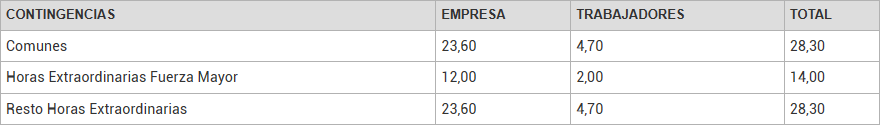
\includegraphics[scale=0.4]{img/Contingencias.png} \\
                \caption{Costes de la empresa - Contingencias comunes}
                \label{Costes de la empresa - Contingencias comunes}
            \end{minipage}
        \end{figure}
        
        \item\textit {Contingencias profesionales y conceptos de recaudación conjunta:}\\
        \begin{enumerate}
            \item\textit {Accidentes de Trabajo (AT):}\\
            Porcentaje que paga la empresa por accidentes de trabajo y enfermedad profesional.\\
            \begin{figure}[h]
              \begin{minipage}{1.3\textwidth}
                \centering
                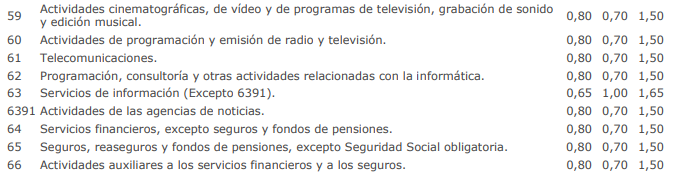
\includegraphics[scale=0.5]{img/AT.png} \\
                \caption{Costes de la empresa - Accidentes de trabajo}
                \label{Costes de la empresa - Accidentes de trabajo}
               \end{minipage}
            \end{figure}
            
            \item\textit {Desempleo:}\\
            Cotización a la seguridad social que paga la empresa por desempleo.\\
            \begin{figure}[h]
              \begin{minipage}{1.3\textwidth}
                \centering
                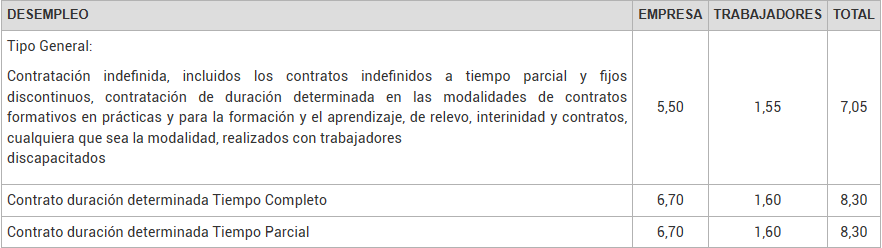
\includegraphics[scale=0.4]{img/Desempleo.png} \\
                \caption{Costes de la empresa - Desempleo}
                \label{Costes de la empresa - Desempleo}
               \end{minipage}
            \end{figure}
            
            \item\textit {Fondo de Garantía Salarial (Fogasa):}\\
            Porcentaje que paga la empresa al Ministerio de Trabajo, Migraciones y Seguridad Social para que, en el caso de declararse la empresa insolvente o en concurso de acreedores, se le paguen a los trabajadores los salarios o indemnizaciones pendientes de abonar.\\
            \begin{figure}[ht]
              \begin{minipage}{1.2\textwidth}
                \centering
                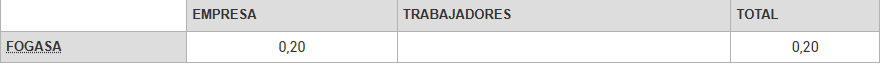
\includegraphics[scale=0.5]{img/Fogasa.png} \\
                \caption{Costes de la empresa - Fogasa}
                \label{Costes de la empresa - Fogasa}
               \end{minipage}
            \end{figure}
            
            \item\textit{} {Formación profesional:}\\
            Cotización que cubre la cuota de necesidades formativas del trabajador.
            \begin{figure}[ht]
              \begin{minipage}{1.2\textwidth}
                \centering
                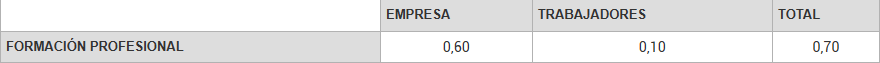
\includegraphics[scale=0.5]{img/FormacionProfesional.png} \\
                \caption{Costes de la empresa - Formación profesional}
                \label{Costes de la empresa - Formación profesional}
               \end{minipage}
            \end{figure}
        \end{enumerate}
    \end{enumerate}
    A continuación, se muestran las tablas de lo que la empresa debería pagar en el caso de contratar al alumno.
     \tablaSmallSinColores{Viabilidad económica - Costes del alumno}{p{5cm} p{4cm} p{4cm}}{Viabilidad económica - Costes del alumno}
        {
          \multicolumn{1}{p{5cm}}{\textbf{Concepto económico}} & \textbf{Coste(€)}\\
         }
         {
        Salario mensual neto & \multicolumn{1}{r}{1950.00€/mes}\\
        Contingencias comunes (23,60\%) & \multicolumn{1}{r}{460.20€/mes}\\
        AT (1,5\%) & \multicolumn{1}{r}{29.25€/mes}\\
        Desempleo (5,50\%)  & \multicolumn{1}{r}{107.25€/mes}\\
        FOGASA (0,20\%) & \multicolumn{1}{r}{3,90€/mes}\\
        Formación profesional (0,60\%) & \multicolumn{1}{r}{11.70€/mes}\\\hline
        \textbf{Salario mensual bruto}  & \multicolumn{1}{r}{2562.10€/mes}\\
        \textbf{Coste 5 meses}  & \multicolumn{1}{r}{12810.5€/5 meses}\\
        }
    No se ha tenido en cuenta la dedicación de los tutores como coste imputable al proyecto puesto que forma parte de las tareas propias de tutorización de la asignatura de proyecto de fin de grado.


    \begin{itemize}
        \item\textit{} {COSTES DE HARDWARE Y SOFTWARE}\\
        Se deben estimar los costes del hardware y software necesario para el desarrollo del proyecto.\\
        Solo deberán tenerse en cuenta en caso de contratación por cuenta ajena, ya que dentro del precio del profesional con cuenta propia vienen incluidos también estos costes.  
        \begin{itemize}
            \item\textit{} {COSTES DE HARDWARE}\\
            Para el desarrollo del TFG se emplea un ordenador portatil ASUS intel CORE i3, un monitor ASUS de 23 pulgadas y como complemento un ratón Logitech.
            Se estima la vida útil de los mismos en 5 años, es decir, cada año se devalúa un 1/5, por lo tanto se calculan las amortizaciones de los meses de uso durante el proyecto (5 meses) de la siguiente manera:


                \tablaSmallSinColores{Costes de hardware y software - Costes de hardware}{p{4cm} p{1cm} p{1cm} p{1cm}}{Costes de hardware y software - Costes de hardware}
                {
                  \multicolumn{1}{p{3cm}}{\textbf{Concepto económico}} &  \multicolumn{1}{p{1cm}}{\textbf{Coste(€)}} & \multicolumn{1}{p{1cm}}\textbf{Amortización(€)} & \multicolumn{1}{p{1cm}}\textbf{Años}\\
                 }
                 {
                Ordenador ASUS & \multicolumn{1}{r}{550}\ & \multicolumn{1}{r}{45,83}\ & \multicolumn{1}{r}{5 años}\\
                Monitor ASUS & \multicolumn{1}{r}{106}\ & \multicolumn{1}{r}{8,83}\ & \multicolumn{1}{r}{5 años}\\
                Ratón LOGITECH & \multicolumn{1}{r}{17,99}\
                 & \multicolumn{1}{r}{1,49}\ & \multicolumn{1}{r}{5 años}\\\hline
                \textbf{Total}  & \multicolumn{1}{r}{673,99} & \multicolumn{1}{r}{56,15} & \multicolumn{1}{r}{5 años}\\
                }

            \item\textit{} {COSTES DE SOFTWARE}\\
            Igualmente, se van a calcular los costes que supone el software que se utiliza para la realización del proyecto, tanto para el despliegue de la aplicación web, como para la base de datos a través de Heroku. También se estimará la vida útil de los mismos en 5 años.

                \tablaSmallSinColores{Trabajador por cuenta ajena - Costes de software}{p{6cm} p{2cm}}{Trabajador por cuenta ajena - Costes de software}
                {
                  \multicolumn{1}{p{6cm}}{\textbf{Concepto económico}} &  \multicolumn{1}{p{2cm}}{\textbf{Coste(€)}} \\
                 }
                 {
                Windows 10 & \multicolumn{1}{r}{1,50}\\
                Heroku app & \multicolumn{1}{r}{7,00}\\
                Heroku PostgreSQL & \multicolumn{1}{r}{9,00}\\\hline
                \textbf{Total}  & \multicolumn{1}{r}{17,50}\\
                }

        \end{itemize}
    \end{itemize}
    \begin{itemize}
    \item\textit{} {COSTES TOTALES}\\
    Se calculan los gastos totales que derivan de la contratación del alumno, la compra de los sistemas hardware y los sistemas software.

    

            \tablaSmallSinColores{Trabajador por cuenta ajena - Costes totales}{p{4cm} p{1cm} p{1cm} p{1cm}}{Trabajador por cuenta ajena - Costes totales}
            {
              \multicolumn{1}{p{3cm}}{\textbf{Concepto económico}} &  \multicolumn{1}{p{1cm}}{\textbf{Coste(€)}} & \multicolumn{1}{p{1cm}}\textbf{Amortización(€)} & \multicolumn{1}{p{1cm}}\textbf{Años}\\
             }
             {
            Coste del alumno & \multicolumn{1}{r}{12810,5}\ & \multicolumn{1}{r}{-}\ & \multicolumn{1}{r}{-}\\
            Coste hardware & \multicolumn{1}{r}{673,99}\ & \multicolumn{1}{r}{87,62}\ & \multicolumn{1}{r}{5 años}\\
            Coste software & \multicolumn{1}{r}{17,50}\
             & \multicolumn{1}{r}{-}\ & \multicolumn{1}{r}{-}\\\hline
            \textbf{Total}  & \multicolumn{1}{r}{13501,99} & \multicolumn{1}{r}{92,04} & \multicolumn{1}{r}{5 años}\\
            }

    \end{itemize}
\end{itemize}


\subsubsection{BENEFICIOS}
La página web se va a distribuir de manera libre y gratuita utilizándose principalmente en la investigación sobre el impacto en Twitter de los Bienes de Interés Cultural del Camino de Santiago Francés en su tramos castellano leonés, por lo que no se generarán beneficios.
La página web tampoco incluye anuncios publicitarios, por lo que tampoco se obtendrán beneficios de los mismos.

\subsection{Viabilidad legal}
Además de estimar los costes que supone la realización del proyecto, se necesitan las licencias del software para cumplir con los requisitos legales.\\
Las herramientas utilizadas en este proyecto pueden verse en la siguiente tabla con sus respectivas versiones y licencias:

\begin{table}[ht!]
    \centering
    \begin{tabular}{c|c|c}
         \hline
         \textbf{Herramientas} & \textbf{Versión} &\textbf{Licencia} \\\hline
         {GitHub} &{3.1.2} &{GNU} \\\hline 
         {Flask} &{2.2.2} &{BSD} \\\hline
         {Leaflet} &{1.8.0} &{BSD 2-Clause Simplified} \\\hline
         {Twitter developer} &{-} &{Licencia de uso } \\\hline
         {Heroku} &{-} &{Licencia de servicio} \\\hline
         {PostgreSQL} &{6.18} &{PostgreSQL License} \\\hline 
         {Bootstrap} &{12.16.1} &{MIT} \\\hline 
         {Plotly} &{5.13.0} &{MIT} \\\hline
         {Pandas} &{1.5.2} &{BSD} \\\hline 
         {Werkzeug} &{9.1.0} &{BSD-3-Clause New} \\\hline
         {Psycopg2} &{2.9.5} &{LGPL} \\\hline 
         {Dotenv} &{0.21.0} &{BSD-2-Clause Simplified} \\\hline 
         {Dateutil} &{2.8.2} &{BSD-3-Clause} \\\hline 
         {Jinja2} &{3.1.2} &{BSD-3-Clause} \\\hline 
         {Sentiment-Analysis-Spanish} &{0.0.25} &{MIT} \\\hline 
         {requests} &{2.28.2} &{Apache 2.0} \\\hline 
    \end{tabular}    \caption{Viabilidad legal - Licencias}
    \label{tab:my_label}
\end{table}

A continuación, se detallan las características de cada una de las licencias nombradas anteriormente y cual es su funcionamiento:\\

\begin{enumerate}
    \item {\textbf{GNU \textit{Git}}\textit{("GNU General Public License")}}\cite{GNU}\\
    Licencia de software libre, la cual permite modificar, utilizar y distribuir código fuente siempre que se incluyan los créditos de autor.
    Además, cualquier cambio o actualización del código fuente debe ser libre y gratuito.
    \item {\textbf{BSD }\textit{("Berkeley Source Distribution")}}\cite{BSD}\\
    Licencia de software libre, la cual permite copiar, modificar y distribuir código fuente siempre que se reserve una copia de la declaración original de derechos de autor.Además, permite el uso del código fuente en software no libre
    \item {\textbf{BSD 2}\textit{("Berkeley Source Distribution 2")}}\cite{BSD2}\\
    Licencia de software libre casi ilimitada, la cual permite copiar, modificar y distribuir código fuente siempre que se incluyan los derechos de autor.
     \item {\textbf{BSD 3 }\textit{("Berkeley Source Distribution 3")}}\cite{BSD3}\\
    Licencia de software libre casi ilimitada, que presenta las restricciones de incluir el texto entero de la licencia y de mencionar los derechos de autor original.
    \item {\textbf{Licencia de uso } \textit{Twitter Developer}}\cite{LicenciaUso}\\
    Licencia que se acepta al comenzar el uso de la API de Twitter, la cual incluye el uso permitido, la responsabilidad legal y la terminación de servicio.
    Además, se deben cumplir las políticas de Twitter, entre ellas las de contenido, privacidad y seguridad.
    \item {\textbf{Licencia de servicio } \textit{Heroku}}\cite{LicenciaServicio}\\
    Licencia que se acepta al comenzar el servicio con Heroku (propiedad de Salesforce), la cual incluye el uso permitido, la responsabilidad legal y la terminación de servicio.
    \item {\textbf{Licencia } \textit{PostgreSQL}}\cite{LicenciaPostgreSQL}\\\
    Licencia similar a MIT o BSD. Se trata de una licencia de código abierto con permisos de uso, modificación, copia y distribución siempre que se incluyan los créditos de autor.
    \item {\textbf{MIT } \textit{("Massachusetts Institute of Technology")}}\cite{MIT}\\
    Se concede el permiso de usar, copiar, modificar, fusionar, publicar, distribuir, sublicenciar y/o vender copias del Software.
    \item {\textbf{LGPL }\textit{("Lesser General Public License")}}\cite{LGPL}\\
    Licencia de software libre que permite la permite copia, distribución o modificación de código fuente; el resto de acciones no estarán cubiertas por esta licencia.
    \item {\textbf{Apache 2.0 }}\cite{Apache}\\
    Licencia de software libre que permite la permite  utilizar, copiar, modificar y distribuir el software, incluyendo una copia de la licencia en la distribución y con la obligación de notificar el uso patentado del software.
\end{enumerate}
La licencia que se ha creido más conveniente para el proyecto ha sido la licencia MIT, ya que es una licencia permisiva que permite a los usuarios realizar diversas acciones incluyendo el uso comercial, la modificación, la distribución y el uso privado, y es compatible con todas las licencias de las herramientas utilizadas en el proyecto.




